% cd /disks/PROJECT/Mickael/COMMUNICATION/SMPGD2016/;
% pdflatex Beamer_SMPGD2016.tex; bibtex Beamer_SMPGD2016; pdflatex Beamer_SMPGD2016.tex; pdflatex Beamer_SMPGD2016.tex
% evince Beamer_SMPGD2016.pdf &

\documentclass[10pt, xcolors={RGB}, hyperref={pdfpagelabels=false,
        colorlinks=true,
        pdftex=true,
        bookmarks=true,
        bookmarksopen=true,
        hyperfootnotes=true}]{beamer}
\pdfpageattr{/Group << /S /Transparency /I true /CS /DeviceRGB>>}
\usepackage[T1]{fontenc}
\usepackage[utf8]{inputenc}
\usepackage{graphicx}
\usepackage{tabularx}
\usepackage{multirow}
\usepackage{pifont}
\usepackage{multicol}
\usepackage{setspace}
\renewcommand{\baselinestretch}{1.5}
\usepackage{helvet}
\renewcommand{\familydefault}{\sfdefault}
\usepackage[square, authoryear]{natbib}

\definecolor{dodgerblue}{RGB}{30,144,255}
\definecolor{springgreen3}{RGB}{0,139,69}
\definecolor{springgreen2}{RGB}{0,205,102}
\definecolor{firebrick2}{RGB}{238,44,44}
\definecolor{maroon2}{RGB}{238,48,167}
\definecolor{goldenrod2}{RGB}{238,180,34}
\definecolor{deepskyblue}{RGB}{0,191,255}



\usetheme{CambridgeUS}
\useoutertheme{infolines}
\useinnertheme{rectangles}
\setbeamercolor{frametitle}{fg=white, bg=springgreen3!90!black!60!white}
\setbeamercolor{title}{fg=white, bg=springgreen3!50!white}
\setbeamercolor{palette primary}{fg=springgreen3!40!black, bg=springgreen3!50!white}
\setbeamercolor{palette secondary}{fg=springgreen3!30!black, bg=springgreen3!70!white}
\setbeamercolor{palette tertiary}{fg=springgreen3!20!black, bg=springgreen3!90!white}
\setbeamercolor{structure}{fg=springgreen3!70!white}
\setbeamercolor{background canvas}{bg=white}
\setbeamercolor{normal text}{fg=black}
\setbeamercolor{block title}{bg=dodgerblue, fg=white!75!dodgerblue}
\setbeamercolor{example text}{fg=springgreen3}
\setbeamercolor{block title example}{bg=springgreen3, fg=white!75!springgreen3}
\setbeamercolor{alerted text}{fg=firebrick2}
\setbeamercolor{block title alerted}{bg=firebrick2, fg=white!75!firebrick2}
\setbeamertemplate{navigation symbols}{}
\addtobeamertemplate{headline}{\hypersetup{allcolors=springgreen3!40!black}}{}

\def\cst#1{\def\@cst{#1}}
\defbeamertemplate*{title page}{custom}[1][]{
    \renewcommand{\baselinestretch}{1.25}
    \begin{centering}
        \begin{beamercolorbox}[sep=3pt,center,#1]{institute}
            \usebeamerfont{institute}{\insertinstitute}
        \end{beamercolorbox}
        \vfill
        \begin{beamercolorbox}[sep=8pt, center, colsep=-4bp, rounded=true, shadow=true, #1]{title}
            \usebeamerfont{title}\inserttitle\par%
            \ifx\insertsubtitle\@empty%
            \else%
            \vskip0.25em%
            {\usebeamerfont{subtitle}\usebeamercolor[fg]{subtitle}\insertsubtitle\par}%
            \fi%
        \end{beamercolorbox}%
        \vskip1em\par
        \begin{beamercolorbox}[sep=8pt,center,#1]{author}
            \usebeamerfont{author}\insertauthor
        \end{beamercolorbox}
        \begin{beamercolorbox}[sep=8pt,center,#1]{cst}
            \usebeamerfont{institute}\@cst
        \end{beamercolorbox}
        \begin{beamercolorbox}[sep=8pt,center,#1]{date}
            \usebeamerfont{date}{\small\insertdate}
        \end{beamercolorbox}
        \vfill
        {\usebeamercolor[fg]{titlegraphic}\inserttitlegraphic\par}
    \end{centering}
    \renewcommand{\baselinestretch}{1.5}
}



\hypersetup{%
    linkcolor=dodgerblue,
    urlcolor=firebrick2,
    citecolor=springgreen3,
    filecolor=goldenrod2,
    menucolor=dodgerblue,
    bookmarksopen=true}
\renewcommand{\thefootnote}{\textcolor{maroon2}{\arabic{footnote}}}

\usepackage{textcomp}
\usepackage{listings}
\usepackage{courier}

\newcommand\bref[2]{\hyperref[#1]{#2~\ref*{#1}}}
\newcommand\cmd[1]{\texttt{\color{black}\textbf{#1}}}
\newcommand\cmdb[1]{\texttt{\color{dodgerblue}\textbf{#1}}}
\newcommand\cmdr[1]{\texttt{\color{firebrick2}\textbf{#1}}}
\newcommand\cmdg[1]{\texttt{\color{springgreen3}\textbf{#1}}}
\newcommand\cmdy[1]{\texttt{\color{goldenrod2}\textbf{#1}}}
\newcommand\blue[1]{{\color{dodgerblue}\textbf{#1}}}
\newcommand\red[1]{{\color{firebrick2}\textbf{#1}}}
\newcommand\green[1]{{\color{springgreen3}\textbf{#1}}}
\newcommand\yellow[1]{{\color{goldenrod2}\textbf{#1}}}
\newcommand\pql{{\rmfamily \textbf{\color{goldenrod2}``}}}
\newcommand\pqr{{\rmfamily \textbf{\color{goldenrod2}''}}}
\newcommand\pq[3]{{\rmfamily \textbf{\color{#3}``}}#1{\rmfamily \textbf{\color{#3}''}} - \textcolor{#3}{#2}}
\newenvironment{bquote}[1]
    {\begin{quotation}
    \vspace{10pt}
    \newcommand{\bqauthor}{\normalfont \begin{quote}\begin{flushright}--- #1\end{flushright}\end{quote}}
    \rmfamily \itshape {\huge\textbf{``}}
    }
    {{\huge\textbf{''}}
    \bqauthor
    \end{quotation}
    }

\usepackage[english, francais]{babel}
% \usepackage[english]{babel}
\selectlanguage{francais}

% \AtBeginSection[]
% {
  % \begin{frame}
    % \frametitle{Sommaire}
    % \tableofcontents[sectionstyle=show/hide, subsectionstyle=show/hide/hide]
  % \end{frame}
% }




\date[SMPGD (February 11-12, 2016)]{%
    {%
        {\scriptsize{%
        {\color{springgreen3!90!white}\blue{S}tatistical \blue{M}ethods for \blue{P}ost \blue{G}enomic \blue{D}ata}\\ \vskip -0.15cm
        {\color{springgreen3!70!white}February 11-12, 2016}%
        }}%
    }%
}

\author[Mickaël Canouil]{%
    \texorpdfstring{%
        \underline{Mickaël Canouil}$^{1}$, Ghislain Rocheleau$^{1}$, Loïc Yengo$^{1}$, Philippe Froguel$^{1,2}$\\
        {\tiny{$^{1}$Univ. Lille, CNRS, Institut Pasteur de Lille, UMR 8199 - EGID, F-59000 Lille, France\\
        $^{2}$Department of Genomics of Common Disease, Imperial College London, London, United Kingdom\\}} %\vskip -0.25cm
        \href{mailto:mickael.canouil@cnrs.fr}{{\scriptsize mickael.canouil@cnrs.fr}}\\\vskip -1em\href{mailto:ghislain.rocheleau@cnrs.fr}{{\tiny \color{black}(ghislain.rocheleau@cnrs.fr)}}%
    }{Mickaël Canouil}
}

% \institute[CNRS UMR 8199]{%
    % {\color{springgreen3!90!white}\blue{I}ntegrated \blue{G}enomics and \blue{M}etabolic \blue{D}iseases \blue{M}odeling
    % \linebreak UMR 8199 (CNRS / Université de Lille 2 / Institut Pasteur de Lille)}%
% }
\institute[CNRS UMR 8199]{%
    {\color{springgreen3!90!white}Integrated Genomics and Metabolic Diseases Modeling
    \linebreak UMR 8199 (CNRS / Université de Lille 2 / Institut Pasteur de Lille)}%
}

\titlegraphic{%
    
\includegraphics[height=1cm, keepaspectratio]{../UTILS/Logos/logo_cnrs.pdf}\hspace{1.5cm}
    
\includegraphics[height=1cm, keepaspectratio]{../UTILS/Logos/UL2-WEB-2014.png}\hspace{1.5cm}
    
\includegraphics[height=1cm, keepaspectratio]{../UTILS/Logos/Institut-Pasteur-de-Lille.png}\hspace{1.5cm}
    
\includegraphics[height=1cm, keepaspectratio]{../UTILS/Logos/logo_egid.pdf}%
}

\newcommand\cb[1]{{\textcolor{dodgerblue}{#1}}}
\title[\texorpdfstring{\color{black}Longitudinal Genetic Modelling}{}]{%
    Longitudinal Genetic Modelling
}

\subtitle{%
    \textit{Revisiting Associations of SNPs Associated with Blood Fasting Glucose in Normoglycemic Individuals}
}

% \cst{{\color{springgreen3!90!white}\textbf{SMPGD}}}

\usepackage[english]{babel}
\selectlanguage{english}

\usepackage{tikz}
% \graphicspath{{figures/}}
\usebackgroundtemplate{%
    % \shorthandoff{;}%
    \tikz\node[opacity=0.10, inner sep=0pt]{%
        
\includegraphics[height=\paperheight, width=\paperwidth]{../UTILS/Background/BG03_Beamer.jpg}%
    };%
}

\setbeameroption{show notes}
\setbeameroption{hide notes}
% \setbeamertemplate{note page}[plain]

\defbeamertemplate{description item}{align left}{\insertdescriptionitem\hfill}
\setbeamertemplate{description item}[align left]

\begin{document}
\maketitle
\note{\par{\green{\ding{110}} First of all, I would like to thank the organizing committee for giving me the opportunity to present my work.}}

% \begin{frame}{\lettrine{S}ommaire}
    % \vspace{-3em}
    % \begin{multicols}{2}
        % \noindent
        % \tableofcontents[sectionstyle=show/show, subsectionstyle=hide/hide/hide, subsubsectionstyle=hide/hide/hide, sections={1-4}]
        % \columnbreak
        % \tableofcontents[sectionstyle=show/show, subsectionstyle=hide/hide/hide, subsubsectionstyle=hide/hide/hide, sections={5-8}]
    % \end{multicols}
% \end{frame}
% \note{\green{\ding{110}} }


\section{Background}
\begin{frame}{\lettrine{B}ackground}
    \begin{itemize}
        \setlength\itemsep{1em}
        \item Genome-wide association studies (GWAS) have been extensively used to identify genetic markers.
        \item Typically, GWAS are based on cross-sectional data.
        \item The recent use of approaches to account for longitudinal data is driven among other things, by the need
        to increase statistical power.
        \item One possible solution is to increase sample size by meta-analysing multiple cohorts \citep{scott_large-scale_2012}.
    \end{itemize}
\end{frame}
\note{%
    \par{\green{\ding{110}} Genome-wide association studies (GWAS) have been extensively used to identify genetic markers.}
    \par{\green{\ding{110}} Typically, GWAS are based on cross-sectional data.}
    \par{\green{\ding{110}} Alternative approach consists in using longitudinal (repeated measures) data, when available.
    These approaches are driven among other things by the need to increase statistical power.}
    \par{\green{\ding{110}} One way to increase power is to increase sample size by meta-analysing multiple cohorts \citep{scott_large-scale_2012}.}
    \par{\green{\ding{110}} Such increase in statistical power is not always reached using repeated measures as we will shown later.}
}


\section{Data}
\begin{frame}{\lettrine{D}ata}
    \begin{itemize}
        \setlength\itemsep{1em}
        \item Metabochip DNA arrays (Illumina) \citep{voight_metabochip_2012} assayed in individuals recruited in the French cohort D.E.S.I.R.\\
        (\textbf{D}onnées \textbf{É}pidémiologiques sur le \textbf{S}yndrome d’\textbf{I}nsulino-\textbf{R}ésistance).
        \item D.E.S.I.R. is a prospective cohort (5,212 individuals) followed up  for 9 years
        (measured at baseline, 3, 6 and 9 years) for many biological traits
        and several pathologies (e.g. type 2 diabetes, cardiovascular diseases, etc.).
    \end{itemize}
\end{frame}
\note{
    \par{\green{\ding{110}} Another solution is to account for repeated measures when available as in the french cohort DESIR.}
    \par{\green{\ding{110}} DESIR is a prospective cohort which includes over five thousands individuals assayed with the Metabochip DNA arrays (Genotypes for 127k SNPs were available for statistical analysis).}
    \par{\green{\ding{110}} Many biological traits were measured at four times (baseline, 3, 6 and 9 years) and several pathologies are available in this cohort.}
}

\begin{frame}{\lettrine{D}ata}
\begin{center}
    \fcolorbox{black}{white}{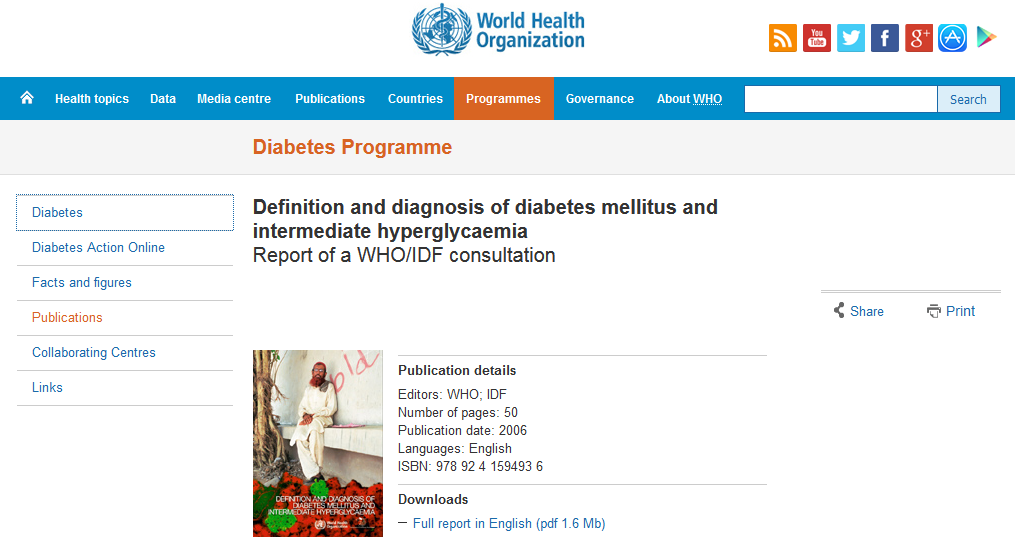
\includegraphics[width=7.5cm]{figures/WHO.png}}
    \par{The focus of this study is on normoglycemic individuals, defined for fasting plasma glucose (FPG) $<$ 7.0 mmol/l \citep{world_health_organization_definition_2006}.}
\end{center}
\end{frame}
\note{
    \par{\green{\ding{110}} We focused, in our study, on normoglycemic individuals, defined for fasting plasma glucose lower than 7.0 mmol/l according to the \cite{world_health_organization_definition_2006}.}
}

\begin{frame}{\lettrine{D}ata}
\par{%
\begin{center}
    \fcolorbox{black}{white}{\begin{minipage}{0.95\textwidth}\input{/disks/DATA/THESE_MC/DESIR_FG_Longitudinal/desir.tex}\end{minipage}}
\end{center}
}
\end{frame}
\note{\par{\green{\ding{110}} DESIR is composed of nearly fifty percent of male and female followed-up, among other things, for the fasting plasma glucose.}}

\begin{frame}{\lettrine{D}ata}
\par{In this table, we focus on fasting plasma glucose measured at baseline, 3, 6 and 9 years (4 measures).}
\begin{center}
    \fcolorbox{black}{white}{\begin{minipage}{0.95\textwidth}\input{/disks/DATA/THESE_MC/DESIR_FG_Longitudinal/desirNA.tex}\end{minipage}}
\end{center}
\end{frame}
\note{\par{\green{\ding{110}} At the end of the follow-up 24 percent of the originally recruited individuals were lost.}}


\section{Methods}
\begin{frame}{\lettrine{M}ethods}
\par{\vspace{-0.75em}{\footnotesize{$Y_i$ is the measured fasting plasma glucose and $G_i$ denotes the genotypes coded 0, 1 or 2.}}
\begin{description}
    \item<1->[Linear Model (Baseline)] \hfill \\\hspace{-5em} $Y_i = \beta_0 + \beta_gG_i + \epsilon_i${\footnotesize{, where $\epsilon_i\sim\mathcal{N}(0, \sigma^2)$}}\\
    \item<2->[Linear Model (Average of $m$ measures)] \hfill \\\hspace{-5em} $\bar{Y}_{i} = \beta_{0} + \beta_gG_i + \epsilon_{i}${\footnotesize{, where $\epsilon_i\sim\mathcal{N}(0, \frac{\sigma^2}{m})$}}\\
    \item<3->[Two-Step] \hfill \\ \vspace{-0.5em}
        \begin{enumerate}\setlength{\itemindent}{-7em}
            \item $Y_{ij} = \beta_{0} + b_{0i} + \beta_{1}t_{ij} + b_{1i}t_{ij} + \epsilon_{ij}${\footnotesize{, where $\epsilon_{ij}\sim{\mathcal{N}}_m(0, V^\dagger{}_i\equiv Z^\dagger{}_iD^\dagger{}Z^\dagger{}_i'+{\sigma^\dagger{}}^2I_m)$}}
            \item $\hat{b}_{0i} = \beta_0^* + \beta_g^*G_i + \epsilon_{i}^*${\footnotesize{, where $\epsilon_{i}^*\sim\mathcal{N}(0, {\sigma^*}^2)$}}
        \end{enumerate}
    \item<4->[Linear Mixed Model (LMM)] \hfill \\\hspace{-5em} $Y_{ij} = \beta_{0} + b_{0i} + \beta_{1}t_{ij} + b_{1i}t_{ij} + \beta_gG_i + \epsilon_{ij}${\footnotesize{, where $\epsilon_{ij}\sim{\mathcal{N}}_m(0, V_i\equiv Z_iDZ_i'+\sigma^2I_m)$}}\\
    \item<5->[Generalised Estimating Equations (GEE)] \hfill \\\hspace{-5em} $\mathbb{E}(Y_i) = \beta_{0} + \beta_{1}t_{ij} + \beta_gG_i$ and $\mathbb{V}(Y_i)=V_i$ (Compound Symmetry).\\
\end{description}
}
\end{frame}
\note{%
    \par{\green{\ding{110}} We compared five approaches from the usual linear regression model to the Linear Mixed Model / Generalised Estimating Equations
    and test for the SNP effect denoted $\beta_g$ for the genotype $G_i$.}
    \par{\green{\ding{110}} The first approach is a simple linear regression model including the genotypes.}
    \par{\green{\ding{110}} The second is similar but the regressed variable is the average of measures by individual.}
    \par{\green{\ding{110}} Another approach is the Two-Step, which consist in performing a linear mixed model without the genotypes in the first step.
    Then get the random intercept estimated and regress it with the genotype.}
    \par{\green{\ding{110}} The usual linear mixed model with random intercept and slope, but without SNP*time interaction.}
    \par{\green{\ding{110}} The last one is the generalised estimating equations model corresponding to the linear mixed model just described.}
}


\section{Results}
\subsection{Top associated SNPs}
\begin{frame}{\lettrine{T}op associated SNPs}
    \begin{center}
        \fcolorbox{black}{white}{\begin{minipage}{0.85\textwidth}\vspace{1em}\input{/disks/DATA/THESE_MC/DESIR_FG_Longitudinal/SMPGD_R0.tex}\end{minipage}}
    \end{center}
    \begin{center}
        \par{{\footnotesize SNPs selected based on \cite{yaghootkar_recent_2013} and \cite{vaxillaire_type_2014}.}}
    \end{center}
\end{frame}
\note{
    \par{\green{\ding{110}} Ten SNPs were selected according to previous findings as reviewed in \cite{yaghootkar_recent_2013}
    and based on results published in Diabetologia \citep{vaxillaire_type_2014} for fasting plasma glucose.}
}

\subsection{Type 1 error}
\begin{frame}{\lettrine{R}esults: Type 1 error}
\vspace{-0.75em}
\par{Type 1 error was computed for 10 SNPs previously shown to be significantly associated with fasting plasma glucose in \cite{vaxillaire_type_2014}.}
\begin{center}
    \par{Testing H0: $\beta_g=0$ versus H1: $\beta_g=d\neq0$}
    \fcolorbox{black}{white}{\includegraphics[width=5.5cm]{/disks/DATA/THESE_MC/DESIR_FG_Longitudinal/Pictures/SMPGD_Type1Error_Intercept.png}}
\end{center}
\par{100,000 genotypes permutations were performed for each selected SNP.}
\end{frame}
\note{
    \par{\green{\ding{110}} In order to check the type 1 error for testing a cross-sectional effect (H0: $\beta_g=0$ versus H1: $\beta_2=d\neq0$),
    for each of the ten selected SNPs, the genotypes were permuted 100,000 times according to the expected $\alpha=5\%$.}
    \par{\green{\ding{110}} Our results show a controlled type 1 error, close to the expected alpha of five percent for all of the five models studied.}
}

\subsection{Statistical power (post-hoc)}
\begin{frame}{\lettrine{R}esults: Statistical power (post-hoc)}
    \begin{center}
        % \fcolorbox{black}{white}{\begin{minipage}{0.65\textwidth}\vspace{1em}\input{/disks/DATA/THESE_MC/DESIR_FG_Longitudinal/SMPGD_R1.tex}\end{minipage}}
        % \fcolorbox{black}{white}{\begin{minipage}{0.65\textwidth}\vspace{1em}\input{/disks/DATA/THESE_MC/DESIR_FG_Longitudinal/SMPGD_R2.tex}\end{minipage}}
        \temporal<2>{%
            \fcolorbox{black}{white}{\begin{minipage}{0.85\textwidth}\vspace{1em}\input{/disks/DATA/THESE_MC/DESIR_FG_Longitudinal/SMPGD_R0.tex}\end{minipage}}%
        }{%
            \fcolorbox{black}{white}{\begin{minipage}{0.85\textwidth}\vspace{1em}\input{/disks/DATA/THESE_MC/DESIR_FG_Longitudinal/SMPGD_R0bold.tex}\end{minipage}}
        }{}
    \end{center}
    \begin{center}
        \par{{\footnotesize SNPs selected based on \cite{yaghootkar_recent_2013} and \cite{vaxillaire_type_2014}.}}
    \end{center}
\end{frame}
\note{
    \par{\green{\ding{110}} A post-hoc statistical power computation was performed on a subset of SNPs.}
    \par{\green{\ding{110}} SNPs on G6PC2, GCK, IKBKAP and TOP1 genes.}
}

\begin{frame}{\lettrine{R}esults: Statistical power (post-hoc)}
    \begin{center}
        \fcolorbox{black}{white}{\includegraphics[width=5.5cm]{/disks/DATA/THESE_MC/DESIR_FG_Longitudinal/Pictures/SMPGD_Power_Intercept_rs560887.png}}
        \fcolorbox{black}{white}{\includegraphics[width=5.5cm]{/disks/DATA/THESE_MC/DESIR_FG_Longitudinal/Pictures/SMPGD_Power_Intercept_rs2908289.png}}
    \end{center}
    \begin{center}\par{100,000 resamplings were performed for each selected SNP.}\end{center}
\end{frame}
\note{
    \par{\green{\ding{110}} Statistical power (post-hoc) curves were computed based on a resampling strategy in each genotypic class (100,000 resamplings were performed), in order to be model-free.}
    \par{\green{\ding{110}} Here is shown the two most significantly associated SNPs with fasting glucose (in genes G6PC2 and GCK).}
    \par{\green{\ding{110}} Due to the highly significant association of SNP in the G6PC2 gene, the statistical power increase is not as high as in the GCK gene.}
    \par{\green{\ding{110}} For these two SNPs, approaches dealing with longitudinal data showed higher power than the cross-sectional approach
    (linear regression at baseline).
    This result is consistent with the usual belief that longitudinal approaches are more powerful than the cross-sectional approach.}
}

\begin{frame}{\lettrine{R}esults: Statistical power (post-hoc)}
    \begin{center}
        \fcolorbox{black}{white}{\includegraphics[width=5.5cm]{/disks/DATA/THESE_MC/DESIR_FG_Longitudinal/Pictures/SMPGD_Power_Intercept_rs16913693.png}}
        \fcolorbox{black}{white}{\includegraphics[width=5.5cm]{/disks/DATA/THESE_MC/DESIR_FG_Longitudinal/Pictures/SMPGD_Power_Intercept_rs6072275.png}}
    \end{center}
\begin{center}\par{100,000 resamplings were performed for each selected SNP.}\end{center}
\end{frame}
\note{
    \par{\green{\ding{110}} But, this belief clearly doesn't hold in all situations as shown for SNPs in IKBKAP and TOP1 genes.}
    \par{\green{\ding{110}} This can be explain by variance parameters for testing SNP's effect $\beta_g\neq0$.}
    \par{\green{\ding{110}} We looked at estimations of variance parameters and developed/derived formulas for the non-centrality parameter in LMM.}
    \par{\green{\ding{110}} Our LMM could be considered as a random intercept and random slope regression model (RIS).}
}


\section{Non-Centrality Parameter \& statistical power}
\begin{frame}{\lettrine{N}on-Centrality Parameter \& statistical power}
\par{%
    Closed-form formulas for testing SNP association under the Cross-Sectional (CS), the Random Intercept (RI) and the Random Intercept and Slope model (RIS)
    \begin{eqnarray}
        NCP_{CS} =& nd^2\left(\frac{2p(1-p)}{\sigma^2}\right)\\[0.25cm]
        NCP_{RI} =& NCP_{CS}\left(\frac{m\sigma^2}{\sigma^2+m\sigma^2_{b0}}\right)\\[0.25cm]
        NCP_{RIS} =& NCP_{RI}U\\[0.25cm]
        \textnormal{with \hspace{1em}} U =& \frac{%
                (\sigma^2+\sigma^2_{b1}\sum^{m}_{j=1}(t_j-\bar{t})^2)(\sigma^2+m\sigma^2_{b0})%
            }{%
                (\sigma^2+\sigma^2_{b1}\sum^{m}_{j=1}(t_j-\bar{t})^2)(\sigma^2+m\sigma^2_{b0})-m\rho^2\sigma^2_{b0}\sigma^2_{b1}\sum^{m}_{j=1}(t_j-\bar{t})^2
            }\geq 1%\\[0.25cm]
    \end{eqnarray}
}
\end{frame}
\note{{\scriptsize
    \par{\green{\ding{110}} We can write $NCP_{RIS}$ as a product of the NCP in the RI model and a factor $U$ always greater than or equal to 1.}
    \par{\green{\ding{110}} This guarantees that the NCP for the RIS model is always greater than or equal to the NCP for the RI model
    but it does not imply that NCP for the RIS model is greater than the NCP under the cross-sectional approach.}
    \newline
    \par{\green{\ding{110}} %
        Where $d$ is the effect size;\\
        $n$ is the sample size (number of individuals);\\
        $m$ is the number of repeated measures;    \\
        $\sigma^2$ is the residual variance;\\
        $\sigma^2_{b0}$ and $\sigma^2_{b1}$ are the variances of the random parameters $b_{0i}$ and $b_{1i}$;\\
        $\rho$ is the correlation coefficient between $b_{0i}$ and $b_{1i}$.}
    }
}

\begin{frame}{\lettrine{N}on-Centrality Parameter \& statistical power}
    \begin{center}
        % \par{\textcolor<2>{maroon2}{This implies that $NCP_{RIS} \geq NCP_{RI}$ but \textbf<2>{\temporal<2>{no guarantee}{\underline{no guarantee}}{\underline{no guarantee}}} that $NCP_{RIS} > NCP_{CS}$}}
        \par{\textcolor<2>{maroon2}{This implies that $NCP_{RIS} \geq NCP_{RI}$ but \temporal<2>{no guarantee}{\textbf{\underline{no guarantee}}}{} that $NCP_{RIS} > NCP_{CS}$}}
    \end{center}
    \vspace{0.25cm}
    \begin{center}
        \temporal<2>{%
            \fcolorbox{black}{white}{\begin{minipage}{0.80\textwidth}\vspace{1em}\input{/disks/DATA/THESE_MC/DESIR_FG_Longitudinal/NCP0.tex}\end{minipage}}%
        }{%
            \fcolorbox{black}{white}{\begin{minipage}{0.80\textwidth}\vspace{1em}\input{/disks/DATA/THESE_MC/DESIR_FG_Longitudinal/NCP.tex}\end{minipage}}%
        }{}
    \end{center}
\end{frame}
\note{%
    \par{\green{\ding{110}} NCP are computed based on estimations provided by Linear Mixed Model and Linear regression Model on the SNPs previously presented.}
    \par{\green{\ding{110}} NCPs showed results consistent with our statistical power simulations.}
}

\begin{frame}{\lettrine{F}uture research}
\begin{itemize}
    \item Characterise parameter space for which $NCP_{RIS}$ is indeed higher than $NCP_{CS}$;
    \newline
    \item Derive formula for the non-centrality parameter when testing SNP*time interaction effect;
    \newline
    \item Check results consistency according to missing data distribution (MCAR, MAR and MNAR).
\end{itemize}
\end{frame}
\note{
    \par{\green{\ding{110}} These results need to be characterise, especially paramer space for which $NCP_{RIS}$ is indeed higher than $NCP_{CS}$.}
    \par{\green{\ding{110}} SNP*time interaction effect begins to be a parameter of concern in the analysis of longitudinal data (as shown in \cite{sikorska_computationally_2014}).}
    \par{\green{\ding{110}} One concern needs to be carefully addressed: the impact of the missing data distribution.}
}

\section{Acknowledgements}
\begin{frame}{\lettrine{A}cknowledgements}
\begin{center}
    \vspace{0.5cm}
    {\huge\par{Thank you for your attention!}}
    \vspace{0.75cm}
    {\scriptsize
        \par{%
            \green{CNRS UMR 8199}\\
            Ghislain Rocheleau\\
            Loïc Yengo\\
            Philippe Froguel\\
        }
        \vspace{1cm}
        \par{%
        \begin{singlespace*}
            \par{\green{Fundings:}\\
                \textit{
                    This work was supported by grants from "European Genomic Institute for Diabetes"\\
                    (E.G.I.D., ANR-10-LABX-46), "European Commission", "Société Francophone du Diabète" and "Lilly".
                }
            }
        \end{singlespace*}
        }
        \vspace{0.75cm}
        \par{%
            
\includegraphics[height=1.5cm, keepaspectratio]{../UTILS/Logos/logo_cnrs.pdf}\hspace{1cm}
            
\includegraphics[height=1.5cm, keepaspectratio]{../UTILS/Logos/UL2-WEB-2014.png}\hspace{1cm}
            
\includegraphics[height=1.5cm, keepaspectratio]{../UTILS/Logos/Institut-Pasteur-de-Lille.png}\hspace{1cm}
            
\includegraphics[height=1.5cm, keepaspectratio]{../UTILS/Logos/logo_egid.pdf}%
        }
    }
\end{center}
\end{frame}
% \note{\green{\ding{110}} }

% \section{References}
\begin{frame}<handout:0|beamer:0>[noframenumbering]{\lettrine{R}eferences}
    \bibliography{SMPGD2016.bib}
\end{frame}

\end{document}